\section{Kết quả và đánh giá}

\subsection{Kết quả hiện thực}

Các thành phần chính của hệ thống đã được hiện thực trong repository:

\begin{table}[H]
\centering
\caption{Trạng thái hiện thực các thành phần}
\label{tab:implementation_status}
\begin{tabularx}{\textwidth}{|l|l|X|}
\hline
\textbf{Thành phần} & \textbf{Trạng thái} & \textbf{Ghi chú} \\
\hline
Backend FastAPI & Hoàn thành & Có lifecycle, CORS, logging và endpoint chính. \\
\hline
Camera worker & Hoàn thành & Đọc camera, xử lý frame, cập nhật API cache. \\
\hline
Face detection & Hoàn thành & Haar Cascade, chọn khuôn mặt lớn nhất. \\
\hline
Face recognition & Hoàn thành & LBPH model, label map JSON, reload model sau đăng ký. \\
\hline
Fuzzy logic & Hoàn thành & Mamdani fuzzy bằng fuzzylite và fallback logic. \\
\hline
Đăng ký khuôn mặt & Hoàn thành & Thu mẫu, lọc chất lượng, train lại LBPH. \\
\hline
Keypad/OLED/Servo & Đã lắp thử & Có ảnh đấu nối thực tế với keypad, OLED, servo và camera USB. \\
\hline
Frontend dashboard & Hoàn thành & Live frame polling, registration, password change. \\
\hline
Benchmark utility & Đã chạy & Đã đo trên Raspberry Pi với camera \texttt{/dev/video0}, thời gian 60 giây. \\
\hline
\end{tabularx}
\end{table}

\subsection{Kết quả API}

Khi backend chạy, Swagger UI tại \texttt{/docs} có thể dùng để kiểm thử API. Các response camera có dạng:

\begin{lstlisting}[language=Python, caption={Các trường chính trong response camera}]
{
    "success": true,
    "mode": "smart_lock",
    "faces_count": 1,
    "detections": [...],
    "timestamp": "...",
    "camera_id": "local_v4l2",
    "fuzzy": {...},
    "registration": {...},
    "frame_base64": "..."
}
\end{lstlisting}

Endpoint \texttt{/api/v1/camera/latest} bỏ qua \texttt{frame\_base64}, phù hợp với trường hợp chỉ cần metadata nhẹ.

\subsection{Kết quả fuzzy logic}

Bộ fuzzy trả về bốn nhóm hành động. Bảng sau mô tả ý nghĩa trong hệ thống:

\begin{table}[H]
\centering
\caption{Ý nghĩa hành động fuzzy trong hệ thống}
\label{tab:fuzzy_action_result}
\begin{tabularx}{\textwidth}{|l|X|}
\hline
\textbf{Action} & \textbf{Xử lý} \\
\hline
\texttt{unlock} & OLED hiển thị access granted và servo mở khóa nếu keypad không đang hoạt động. \\
\hline
\texttt{otp} & Hiện tại được ghi nhận là trạng thái yêu cầu xác thực bổ sung; phần OTP thực tế chưa được triển khai. \\
\hline
\texttt{deny} & Từ chối truy cập, vẫn hiển thị thông tin nhận diện/rủi ro. \\
\hline
\texttt{lockout} & Đánh dấu rủi ro cao; có thể mở rộng thành cảnh báo hoặc khóa hệ thống. \\
\hline
\end{tabularx}
\end{table}

\subsection{Kết quả giao diện}

Frontend hiển thị được:

\begin{itemize}
    \item trạng thái live/disconnected,
    \item frame camera mới nhất,
    \item số khuôn mặt,
    \item danh tính nhận diện,
    \item hành động fuzzy và phần trăm rủi ro,
    \item thông số LBPH distance, illumination và facial angle,
    \item form đăng ký khuôn mặt,
    \item form đổi mật khẩu keypad.
\end{itemize}

\begin{figure}[H]
    \centering
    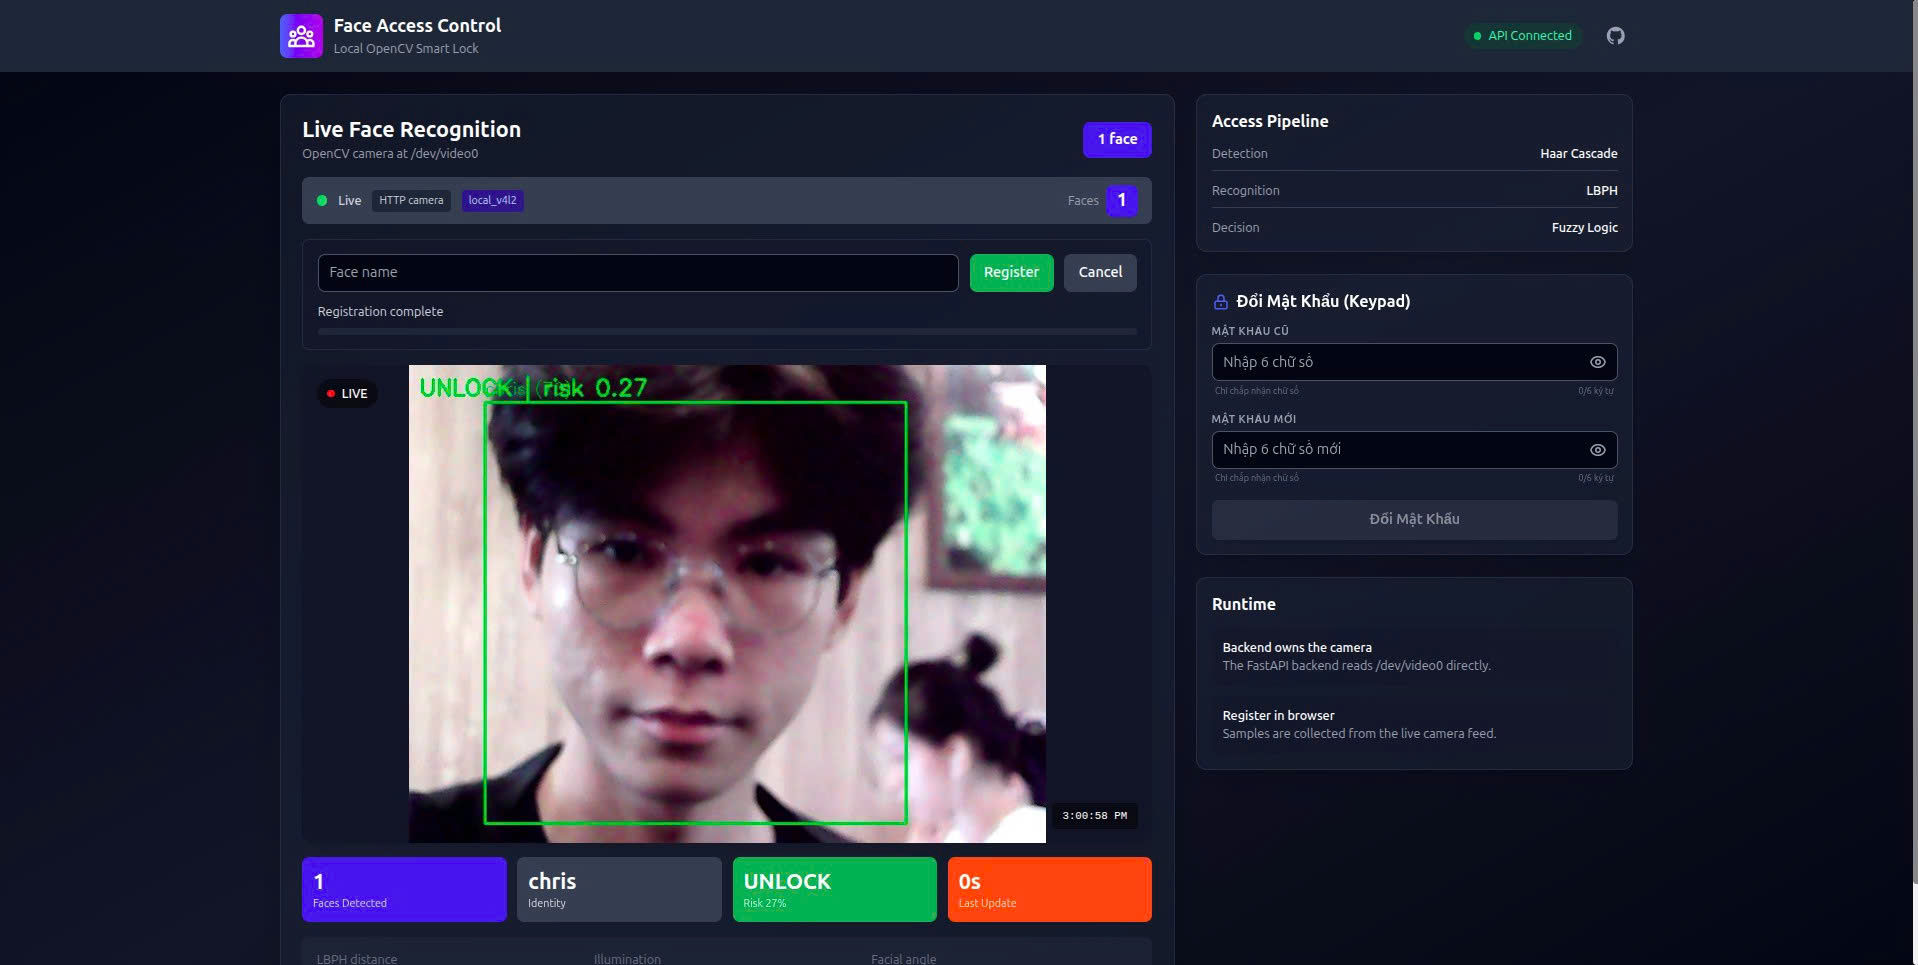
\includegraphics[width=\linewidth]{dashboard_nextjs.png}
    \caption{Kết quả giao diện live face recognition trên dashboard}
    \label{fig:frontend_result}
\end{figure}

\begin{figure}[H]
    \centering
    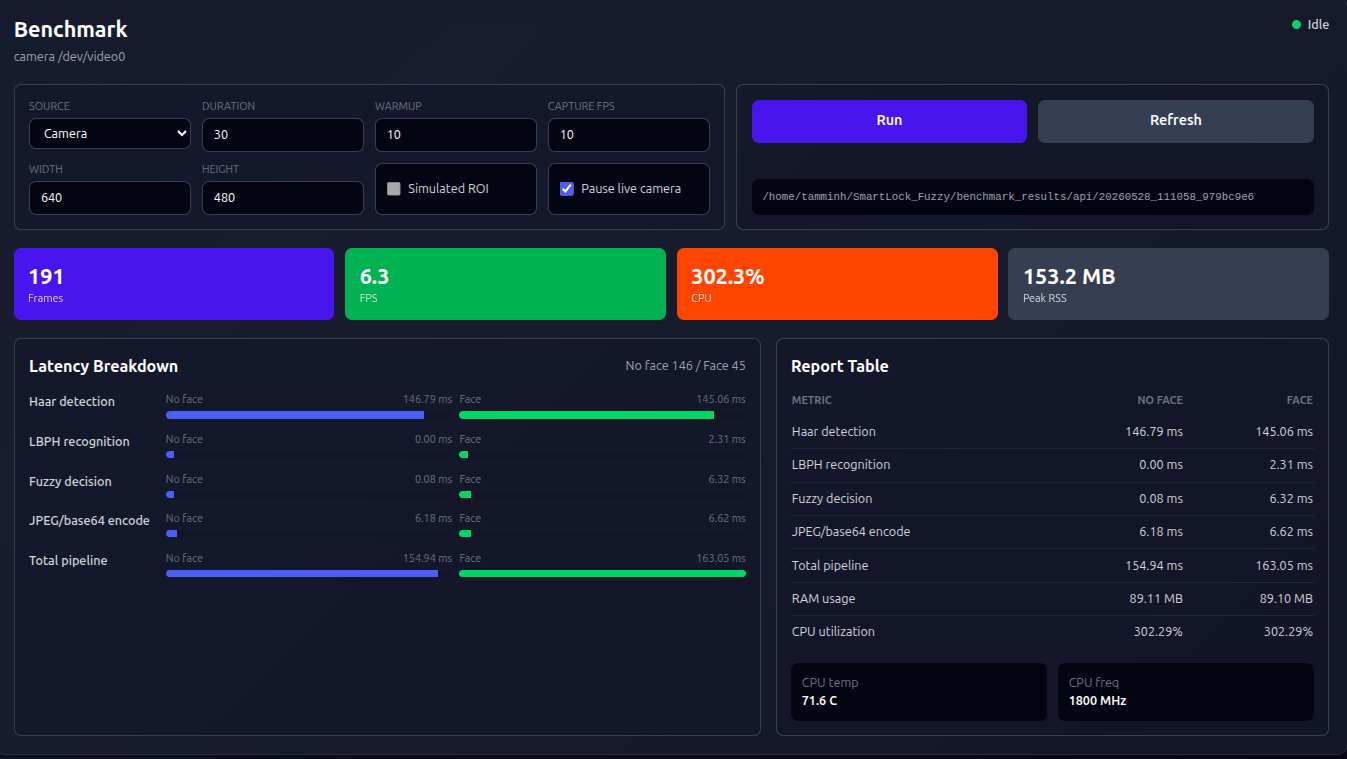
\includegraphics[width=\linewidth]{benchmark_ui.png}
    \caption{Giao diện benchmark hiển thị FPS, CPU, RAM và độ trễ từng bước}
    \label{fig:benchmark_ui_result}
\end{figure}

\subsection{Kết quả phần cứng}

Hệ thống đã được lắp trên Raspberry Pi cùng camera USB, keypad ma trận 4x4, OLED SSD1306 và servo. Ảnh ở Hình \ref{fig:hardware_connected_result} cho thấy cấu hình kết nối thực tế: camera gắn qua USB, keypad nối vào các chân GPIO hàng/cột, OLED nối qua SPI và servo nhận tín hiệu PWM từ GPIO18. Servo được cấp nguồn 5V ngoài và nối chung GND với Raspberry Pi để tránh sụt áp khi motor quay.

\begin{figure}[H]
    \centering
    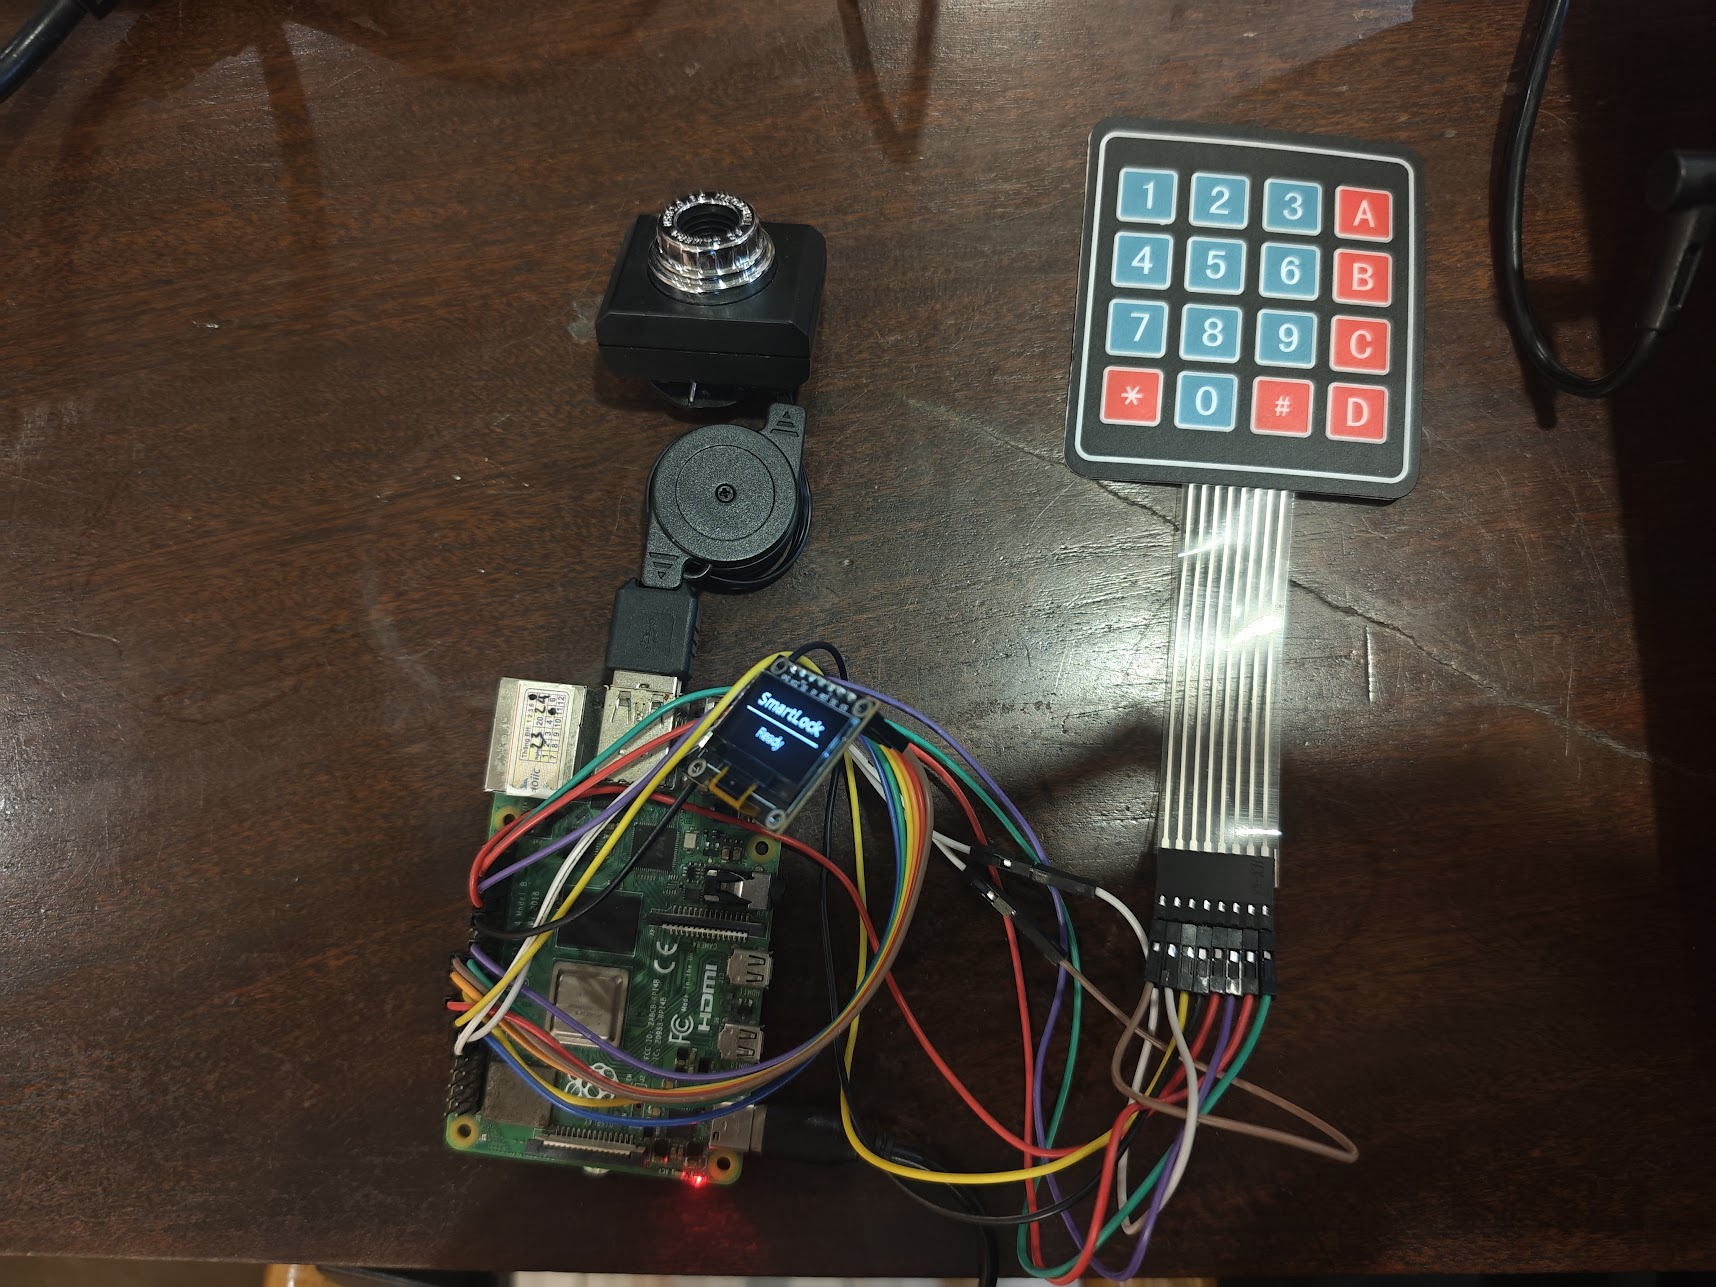
\includegraphics[width=\linewidth]{schematic_connected.png}
    \caption{Mạch phần cứng đã đấu nối trên Raspberry Pi}
    \label{fig:hardware_connected_result}
\end{figure}

Trong quá trình chạy thử, OLED hiển thị trạng thái \texttt{SmartLock Ready}; keypad được dùng cho kênh xác thực PIN; servo đóng vai trò cơ cấu chốt khóa. Phần mềm phần cứng đã bao gồm quét keypad bằng interrupt, chống dội phím, lockout sau nhiều lần nhập sai và đưa duty cycle servo về 0 sau khi quay để giảm rung.

\subsection{Benchmark và giới hạn kiểm chứng}

Benchmark được chạy trực tiếp trên thiết bị edge Raspberry Pi với camera \texttt{/dev/video0}, độ phân giải $640\times480$, FPS capture đặt 10, thời gian đo 60 giây và 20 frame warm-up. Tổng cộng script ghi nhận 489 frame, trong đó có 435 frame không có mặt và 54 frame có mặt; không có frame bị drop. Throughput trung bình đạt 8.14 FPS. Nhiệt độ CPU cuối quá trình đo là $67.7^\circ$C, xung CPU 1800 MHz và cờ throttling là \texttt{0x0}, cho thấy thiết bị không bị throttling trong lần đo này.

\begin{table}[H]
\centering
\caption{Kết quả benchmark pipeline trên Raspberry Pi}
\label{tab:benchmark_results}
\begin{tabular}{|l|c|c|}
\hline
\textbf{Chỉ số} & \textbf{Không có mặt} & \textbf{Có mặt} \\
\hline
Face detection latency & 111.26 ms & 108.43 ms \\
\hline
Face recognition latency & 0.00 ms & 2.15 ms \\
\hline
Fuzzy decision latency & 0.08 ms & 5.90 ms \\
\hline
JPEG/base64 encode latency & 5.91 ms & 6.34 ms \\
\hline
Total pipeline latency & 121.36 ms & 127.36 ms \\
\hline
RAM usage & 89.27 MB & 89.25 MB \\
\hline
CPU utilization & 319.07\% & 319.07\% \\
\hline
\end{tabular}
\end{table}

Kết quả cho thấy phần tốn thời gian nhất là Haar Cascade, chiếm hơn 100 ms mỗi frame ở cả hai trường hợp. Khi có khuôn mặt, hệ thống phát sinh thêm chi phí LBPH và fuzzy decision, nhưng tổng độ trễ chỉ tăng từ 121.36 ms lên 127.36 ms. Với throughput khoảng 8 FPS, pipeline đủ dùng cho kịch bản khóa cửa, nơi yêu cầu chính là phản hồi ổn định trong khoảng dưới một giây thay vì video FPS cao.

Các giới hạn hiện tại:

\begin{itemize}
    \item LBPH nhạy với điều kiện ánh sáng và chất lượng dữ liệu đăng ký.
    \item Fuzzy angle estimation chỉ dựa trên bất đối xứng sáng, chưa phải ước lượng pose thật.
    \item Mật khẩu keypad chưa được lưu bền vững qua các lần restart.
    \item CORS đang mở \texttt{allow\_origins=["*"]}, phù hợp demo nhưng cần siết lại nếu triển khai thật.
    \item Chưa có authentication cho API quản trị như đăng ký khuôn mặt hoặc đổi PIN.
\end{itemize}
